\section{Durchführung}
\label{sec:Durchführung}

In diesem Versuch werden verschiedene Kurven mithilfe eines XY-Schreibers aufgenommen.
Das Schaltbild des Aufbaus ist in \autoref{fig:Abb_5} dargestellt.
\begin{figure}[H]
    \centering
    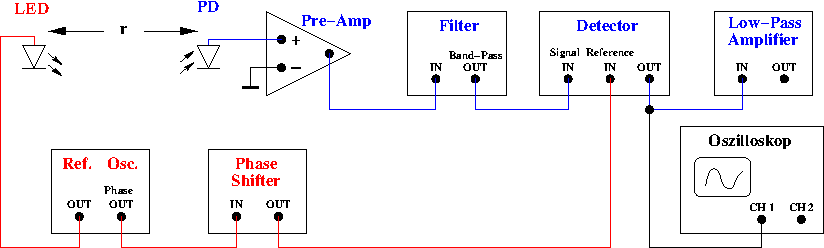
\includegraphics[width=0.8\textwidth]{build/Abb_5.pdf}
    \caption{Schematische Darstellung der Schaltung des Franck-Hertz-Versuchs\cite{V601}.}
    \label{fig:Abb_5}
\end{figure}
Zusätzlich zum in \autoref{subsec:AufAbTheo} beschriebenen Aufbau wird außer dem XY-Schreiber noch ein Heizgenerator mit Thermometer,
Gleichspannungsquellen und ein Picoamperemeter benötigt.
Die Geräte werden wie in \autoref{fig:Abb_5} verschaltet.\\

An der Apparatur kann die Bremsspannung $U_A$ zwischen $\qty{0}{\volt}$ und $\qty{11}{\volt}$ variiert werden.
Auch die Beschleunigungsspannung $U_B$ kann variiert werden, in einem Bereich zwischen $\qty{0}{\volt}$ und $\qty{60}{\volt}$.\\

Vor der ersten Messung wird der XY-Schreiber eingestellt.
Die Besschleunigungsspannung liegt hierbei am X-Eingang an und die Bremsspannung, welche proportional zum Auffängerstrom ist, liegt am Y-Eingang an.
Die Beschleunigungsspannung wird auf konstante $\qty{11}{\volt}$ eingestellt und die Bremsspannung kontinuierlich erhöht.
Der XY-Schreiber nimmt somit den Verlauf des Auffängerstroms in Abhängigkeit von der Bremsspannung auf.
Die Messung wird zunächst mit geschlossenem Stift vom XY-Schreiber aufgenommen und die X- und Y-Achse so angepasst, dass der 
Verlauf der Kurve optimal auf dem Papier zu sehen ist. Dann wird die Kappe entfernt und der Verlauf aufgenommen.
Die Messung wird bei Raumtemperatur durchgeführt.
Eine zweite Messung erfolgt nachdem die Apparatur auf eine Temperatur zwischen $\qty{140}{\celsius}$ und $\qty{160}{\celsius}$
aufgeheizt wird. Die Y-Achse muss hierbei erneut kalibriert werden.
Außerdem wird ohne angeschlossene Quelle am Y-Eingang die Skalierung der X-Achse auf dem Papier eingetragen, indem die Bremsspannung
in $\qty{1}{\volt}$ Abständen erhöht wird und Markierungen gesetzt werden.\\

Im zweiten Teil des Versuchs werden Franck-Hertz-Kurven aufgenommen. 
Diesmal wird die Beschleunigungsspannung variiert, während die Bremsspannung auf konstante $\qty{1}{\volt}$ eingestellt wird.
Am X-Eingang des XY-Eingangs wird die Bremsspannnung angelegt.
Mithilfe des Heizgenerators wird die Temperatur der Apparatur möglichst konstant auf einem Wert zwischen $\qty{160}{\celsius}$
und $\qty{200}{\celsius}$ gehalten.
Der XY-Schreiber muss eventuell neu kalibriert werden. 
Es werden für zwei verschiedene Temperaturen im Bereich Franck-Hertz-Kurven mit dem XY-Schreiber aufgenommen indem die Beschleunigungsspannung
kontinuierlich erhöht wird.
Auch hier wird im Anschluss die X-Achse skaliert.\\



